\subsubsection{Empirical Comparison}
% \begin{table}[t]
% % \begin{wraptable}{R}{0.5\linewidth}
% \caption{The performance comparison of LLMs for code generation on the MBPP \cite{austin2021program} benchmark, measured by \texttt{Pass@1}. For models with various sizes, we report only the largest size version of each model with the magnitude of \texttt{B} parameters.}
% \label{tab:performance_mbpp}
% \centering
% \scalebox{0.75}{
% \rotatebox{0}{
%     \begin{tabular}{lrc}
%     \toprule
%     \textbf{Model} & \textbf{Size} & \texttt{pass@1} \\ 
% \midrule
%     % GPT-4  & - &    \\ 
%     GPT-3.5-Turbo \cite{gpt-3.5-turbo} & - & 52.2   \\
%     Claude-3-Opus \cite{claude3} & - & 86.4 \\
%     Claude-3-Sonnet \cite{claude3} & - & 79.4 \\
%     Claude-3-Haiku \cite{claude3} & - & 80.4 \\
%     \midrule
%     Codestral & 22B & 78.2 \\
%     Qwen2.5-Coder-Instruct & 7B & 83.5 \\
%     Qwen2.5-Coder & 7B & 76.9 \\
%     StarCoder2-Instruct \cite{starcoder2instruct} &  15.5B  & 75.2 \\
%     CodeGemma-Instruct \cite{codegemma_2024}  & 7B  & 54.2 \\
%     CodeGemma \cite{codegemma_2024}  & 7B  & 56.2 \\
%     StarCoder 2 \cite{lozhkov2024starcoder}  & 15B & 66.2 \\
%     WaveCoder \cite{yu2023wavecoder} & 6.7B & 74.9 \\
%     CodeFuse \cite{liu2023mftcoder} & 34B & 61.0    \\
%     CodeShell & 7B & 38.65 \\
%     CodeQwen1.5-Chat \cite{codeqwen} & 7B & 77.7 \\
%     CodeQwen1.5 \cite{codeqwen} & 7B & 72.2 \\
%     Magicoder$S$-CL \cite{wei2023magicoder} & 7B & 68.4 \\
%     Magicoder-CL \cite{wei2023magicoder} & 7B & 64.2 \\
%     DeepSeek-Coder-Instruct \cite{guo2024deepseek} & 33B & 70.0 \\
%     DeepSeek-Coder \cite{guo2024deepseek} & 33B & 66.0 \\
%     WizardCoder \cite{luo2023wizardcoder} & 33B & 78.9   \\
%     phi-1 \cite{gunasekar2023textbooks} & 1.3B & 55.5   \\
%     Code Llama-Instruct \cite{roziere2023code} & 70B & 62.2 \\
%     Code Llama \cite{roziere2023code} & 70B & 62.4    \\
%     CodeGeeX2 \cite{zheng2023codegeex} & 6B & 24.37 \\
%     CodeGeeX \cite{zheng2023codegeex} & 13B & 24.4   \\
%     PanGu-Coder \cite{christopoulou2022pangu} & 2.6B & 23.0 \\
%     CodeGen-NL \cite{nijkamp2022codegen} & 16.1B & 10.92  \\
%     CodeGen-Multi \cite{nijkamp2022codegen} & 16.1B & 20.94  \\
%     CodeGen-Mono \cite{nijkamp2022codegen} & 16.1B & 35.28  \\
%     StarCoder \cite{li2023starcoder} & 5.5B & 52.7  \\
%     CodeT5+ \cite{wang2021codet5} & 16B & 56.6 \\
%     SantaCoder \cite{allal2023santacoder} & 1.1B & 35  \\
%     InCoder \cite{fried2022incoder} & 6.7B & 21.3   \\
%     PolyCoder \cite{xu2022systematic} & 2.7B & 4.39   \\
%     CodeParrot \cite{tunstall2022natural} & 1.5B & 1.29   \\
%     \bottomrule
%     \end{tabular}
% }
% }
% % \end{wraptable}
% \end{table}

\begin{figure*}[t]
\centering
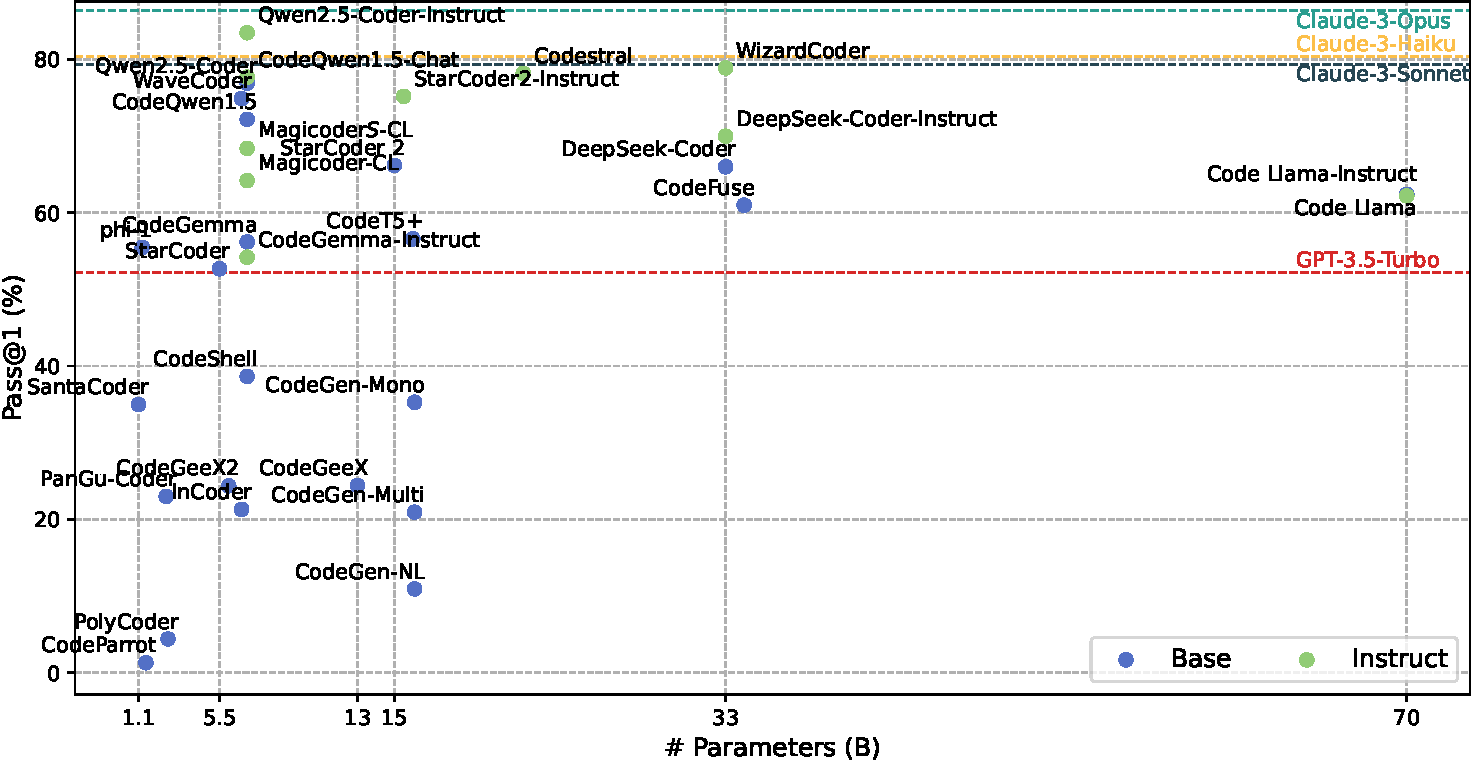
\includegraphics[width=\linewidth]{images/mbpp_scatter.pdf}
\caption{\done{The performance comparison of LLMs for code generation on the MBPP \cite{austin2021program} benchmark, measured by \texttt{Pass@1}. For models with various sizes, we report only the largest size version of each model with a magnitude of \texttt{B} parameters.} 
}
\label{fig:mbpp_performance}
\end{figure*}
% \begin{table}[t] 
% % \begin{wraptable}{R}{0.5\linewidth}
% \caption{
% % The Performance (\texttt{Pass@1}, \texttt{Pass@10}, and \texttt{Pass@100}) comparison of LLMs for code generation on HumanEval benchmark. For the model with various model size, we only report the largest size version of each model.
% \revise{The performance comparison of LLMs for code generation on the HumanEval \cite{chen2021evaluating} benchmark, measured by \texttt{Pass@1}. 
% % Due to the limitations of computational resources we faced, we directly cite the experimental results from the original papers or widely recognized open-source leaderboard in research community.
% For models with various sizes, we report only the largest size version of each model with the magnitude of \texttt{B} parameters. $^\ddag$ denotes instruction-tuned models.
% % DeepSeek-Coder-V2-Instruct is an open-source Mixture-of-Experts (MoE) code language
% % model, which has 236B parameters with only 21B activation parameters. 
% } 
% }
% \label{tab:performance_bigcodebench}
% \centering
% \scalebox{0.82}{
% \rotatebox{0}{
%     \begin{tabular}{clrc}
%     \toprule
%     & \textbf{Model} & \textbf{Size} & \texttt{Full pass@1} \\ 
% \midrule
%     \multirow{10}{*}{\textbf{Closed Source}} 
%          & GPT-4o-0513 \cite{gpt-4o} & - & 51.1 \\
%          & GPT-4-Turbo-0409 \cite{gpt-4-turbo} & - & 48.2 \\
%          & GPT-4-0613 \cite{achiam2023gpt}& - & 46  \\
%          & GPT-3.5-Turbo-0125 \cite{gpt-3.5-turbo}& - & 39.1 \\
%          & Claude-3.5-Sonnet \cite{claude3} & - & 46.8 \\
%          & Claude-3-Opus \cite{claude3} & - & 45.5 \\
%          & Claude-3-Sonnet \cite{claude3} & - & 42.7 \\
%          & Claude-3-Haiku \cite{claude3} & - & 39.4 \\
%          & Gemini-1.5-Pro \cite{reid2024gemini} & - & 43.8 \\
%          & Gemini-1.5-Flash \cite{reid2024gemini} & - & 43.5 \\
%          \midrule
%     \multirow{11}{*}{\textbf{Open Source}} 
%          & $^\ddag$Codestral \cite{codestral} & 22B & 41.8 \\
%          & $^\ddag$DeepSeek-Coder-V2-Instruct \cite{zhu2024deepseek}  & 21B (236B) & 48.2 \\
%          & $^\ddag$Qwen2.5-Coder-Instruct \cite{hui2024qwen2} & 7B & 40.4 \\
%          & $^\ddag$StarCoder2-Instruct \cite{starcoder2instruct} &  15.5B  & 37.6 \\
%          & $^\ddag$CodeGemma-Instruct \cite{codegemma_2024}  & 7B  & 32.3 \\
%          & $^\ddag$WaveCoder-Ultra \cite{yu2023wavecoder} & 6.7B & 33.9 \\
%          & $^\ddag$CodeQwen1.5-Chat \cite{codeqwen} & 7B & 39.6 \\
%          & $^\ddag$Magicoder-S-DS \cite{wei2023magicoder} & 7B & 36.2 \\
%          & $^\ddag$DeepSeek-Coder-Instruct \cite{guo2024deepseek} & 33B & 42 \\
%          & $^\ddag$Phi-3-Medium-128K-Instruct \cite{abdin2024phi} & 14B & 36.8 \\
%          & $^\ddag$Code Llama-Instruct \cite{roziere2023code} & 70B & 40.7 \\
%          & $^\ddag$CodeGeeX4 \cite{zheng2023codegeex} & 9B & 40 \\
%     \bottomrule
%     \end{tabular}
% }
% }
% \vspace{-10pt}
% % \end{wraptable}
% \end{table}

\begin{figure*}[t]
\centering
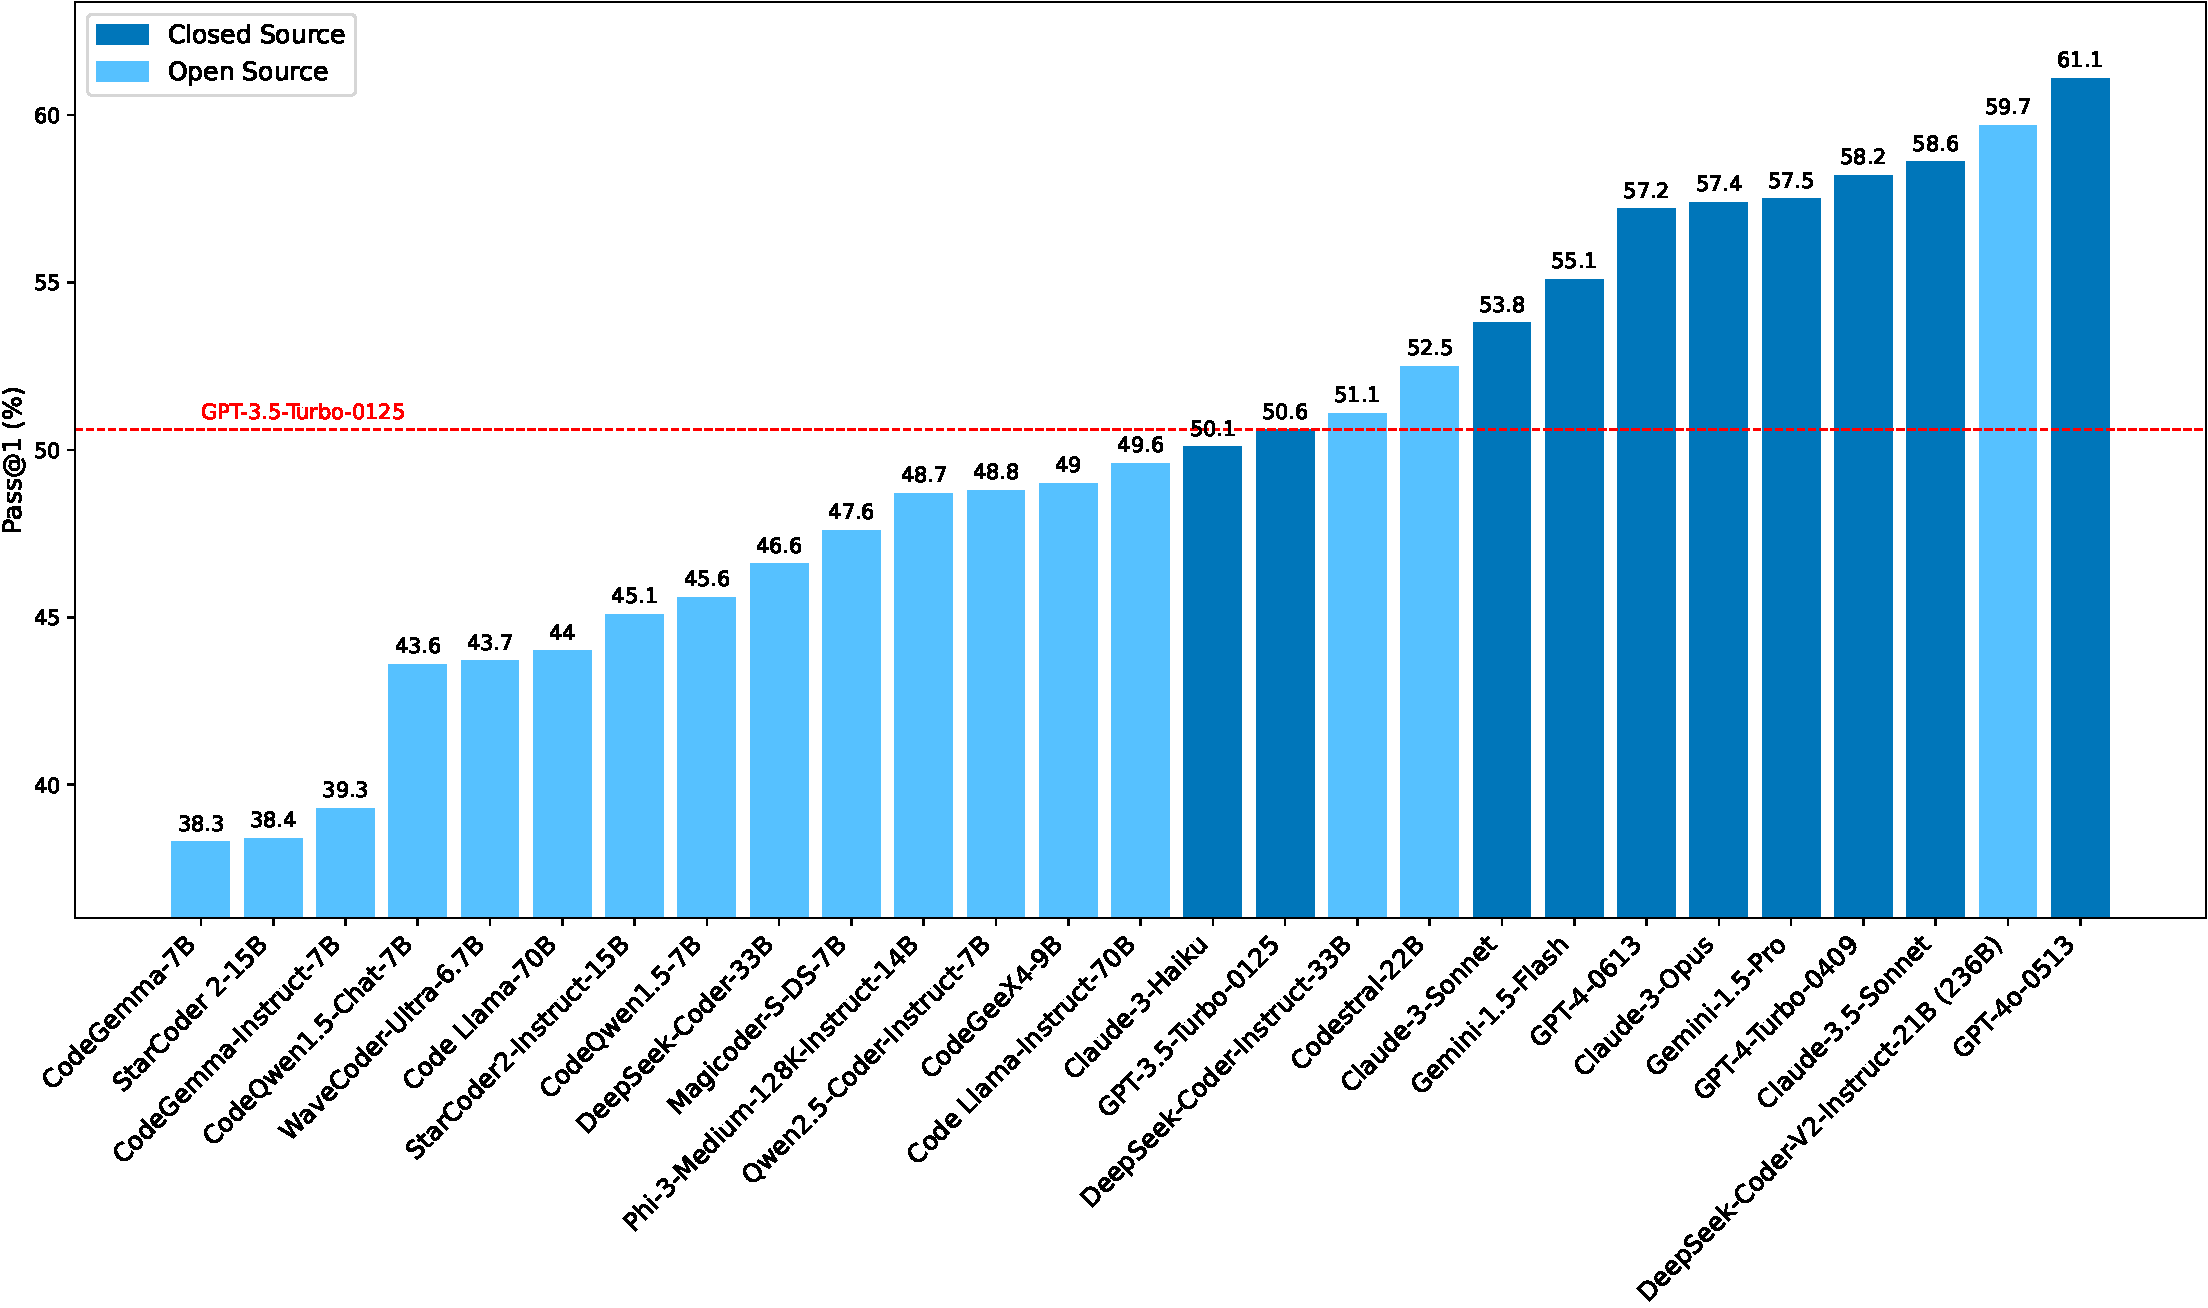
\includegraphics[width=\linewidth]{images/bigcodebench_complete_bar.pdf}
\caption{\done{The performance comparison of LLMs for code generation on the BigCodeBench \cite{zhuo2024bigcodebench} benchmark, measured by \texttt{Pass@1}. For models with various sizes, we report only the largest size version of each model with a magnitude of \texttt{B} parameters.} 
}
\label{fig:bigcodebench_performance}
\end{figure*}
% In this Section, we provide an the performance comparision of LLMs for code generaiton on the widely recognized HumanEval and MBPP benchmarks, as well as the more practical and challenging BigCodeBench benchmar, to highlight the progressive enhancements in LLM capabilities for code generation.
% These three benchmarks can be used to assess a LLM's capability in code generation from different difficulty level and scope of the programming tasks. 
% To be specific, HumanEval is more focused on complex code generation, while MBPP targets basic programming tasks, BigCodeBench focuses on practical and challenging programming tasks.
In this section, we present a performance comparison of LLMs for code generation using the well-regarded HumanEval, MBPP, and the more practical and challenging BigCodeBench benchmarks. 
This empirical comparison aims to highlight the progressive enhancements in LLM capabilities for code generation. 
These benchmarks assess an LLM's ability to generate source code across various levels of difficulty and types of programming tasks. 
Specifically, HumanEval focuses on complex code generation, MBPP targets basic programming tasks, and BigCodeBench emphasizes practical and challenging programming tasks.

% Due to the limitations of computational resources we faced, we directly cite the experimental results from the original papers or widely recognized open-source leaderboard in research community.
% We report the performance on HumanEval with the \texttt{pass@1} as shown in Table \ref{tab:performance_humaneval}, while MBPP and BigCodeBench with \texttt{pass@1}, as shown in Figure \ref{fig:mbpp_performance} and \ref{fig:bigcodebench_performance}, respectively.
Due to the limitations in computational resources we faced, we have cited experimental results from original papers or widely recognized open-source leaderboards within the research community, such as the HumanEval Leaderboard \footnote{\href{https://paperswithcode.com/sota/code-generation-on-humaneval}{https://paperswithcode.com/sota/code-generation-on-humaneval}}, EvalPlus Leaderboard \footnote{\href{https://evalplus.github.io/leaderboard.html}{https://evalplus.github.io/leaderboard.html}}, Big Code Models Leaderboard  \footnote{\href{https://huggingface.co/spaces/bigcode/bigcode-models-leaderboard}{https://huggingface.co/spaces/bigcode/bigcode-models-leaderboard}}, and BigCodeBench Leaderboard \footnote{\href{https://bigcode-bench.github.io/}{https://bigcode-bench.github.io/}}. 
We report performance on HumanEval using the \texttt{pass@1} metric, as shown in Table \ref{tab:performance_humaneval}, while MBPP and BigCodeBench results are presented with \texttt{pass@1} in Figures \ref{fig:mbpp_performance} and \ref{fig:bigcodebench_performance}, respectively.

We offer the following insights:
\begin{itemize}
    % \item The performance gap between open-source and closed-source models on three benchmarks is gradually narrowing. For example, on HumanEval benchmark, DeepSeek-Coder-V2-Instruct with only 21B activation parameters and Qwen2.5-Coder-Instruct \cite{hui2024qwen2} 7B achieves 90\% and 88.4\% pass@1 performance, respectively, which are comparable to much large closed source LLMs Claude-3.5-Sonnet with 92.0\% pass@1 performance. 
    % On MBPP benchmark, Qwen2.5-Coder-Instruct 7B with 83.5\% pass@1 significantly outperforms GPT-3.5-Turbo with 52.2\% pass@1 and achieve a very close performance compared to powerful closed-source Claude-3-Opus with 86.4\% pass@1. On more practical and challenging benchmark BigCodeBench, DeepSeek-Coder-V2-Instruct with 48.2\% surpasses all compared closed source LLMs except equal to GPT-4-Turbo-0409 with 48.2\% and lag behind GPT-4o-0513 with 51.1\%. 
    \item The performance gap between open-source and closed-source models across the three benchmarks is gradually narrowing. For instance, on the HumanEval benchmark, DeepSeek-Coder-V2-Instruct with 21B activation parameters and Qwen2.5-Coder-Instruct 7B achieve 90\% and 88.4\% pass@1, respectively. 
    These results are comparable to the much larger closed-source LLMs, such as Claude-3.5-Sonnet, which achieves 92.0\% pass@1. 
    On the MBPP benchmark, Qwen2.5-Coder-Instruct 7B with 83.5\% pass@1 significantly outperforms GPT-3.5-Turbo with 52.2\% pass@1 and closely rivals the closed-source Claude-3-Opus with 86.4\% pass@1. 
    On the BigCodeBench, DeepSeek-Coder-V2-Instruct achieves 59.7\%, surpassing all compared closed-source and open-source LLMs except for slightly falling behind GPT-4o-0513, which achieves 61.1\%.
    % \item In general, as the model parameters increase, the performance of the Code LLMs improves. However, we observe that Qwen2.5-Coder-Instruct 7B obtain 88.4 pass@1 results, outperforming StarCoder2-Instruct 15.5B with 72.6\% pass@1, DeepSeek-Coder-Instruct 33B with 79.3\% pass@1, and Code Llama-Instruct 70B with 67.8\% pass@1 by a large margin on HumanEval benchmark. We also observe consistent phonomenon across other two benchmarks. 
    % We speculate that Code LLMs with 7B parameters may be enough capable on the code generation task.
    \item Generally, as the number of model parameters increases, the performance of code LLMs improves. However, Qwen2.5-Coder-Instruct 7B achieves 88.4\% pass@1, outperforming larger models like StarCoder2-Instruct 15.5B with 72.6\% pass@1, DeepSeek-Coder-Instruct 33B with 79.3\% pass@1, and Code Llama-Instruct 70B with 67.8\% pass@1 on the HumanEval benchmark. Similar trends are observed across the other two benchmarks, suggesting that code LLMs with 7B parameters may be sufficiently capable for code generation task.
    % \item Compared to base (pretrained) models, their instruction-tuned counterpart consistently achieve better performance across all benchmarks. 
    % For example, on three benchmarks, Qwen2.5-Coder-Instruct outperforms Qwen2.5-Coder by average 21\%,  StarCoder2-Instruct improve StarCoder2 by average 50\%, CodeGemma-Instruct improve CodeGemma by average 25\%, DeepSeek-Coder-Instruct surpass DeepSeek-Coder by average 30\%, and Code Llama-Instruct improve Code Llama by average 80\%. 
    % It verifies the effectiveness of instruction tuning. However, the quality of instruction tuning dataset has significant impact on the model performance \cite{luo2023wizardcoder}.    
    % \item Instruction-tuned models consistently outperform their base (pretrained) counterparts across HumanEval and MBPP benchmarks.
    % For example, 
    % Qwen2.5-Coder-Instruct outperforms Qwen2.5-Coder by an average of 26.04\%, 
    % StarCoder2-Instruct improves StarCoder2 by an average of 35.20\%, 
    % CodeGemma-Instruct improves CodeGemma by an average of 11.26\%, 
    % DeepSeek-Coder-Instruct surpasses DeepSeek-Coder by an average of 23.71\%, and 
    % Code Llama-Instruct improves Code Llama by an average of 13.8\%. The detailed results are illustrated in Table \ref{tab:instruct_improve}.
    % This underscores the effectiveness of instruction tuning, though the quality of the instruction tuning dataset significantly impacts model performance \cite{luo2023wizardcoder,zhou2024lima}.
    \item Instruction-tuned models consistently outperform their base (pretrained) counterparts across the HumanEval and MBPP benchmarks. For instance, Qwen2.5-Coder-Instruct surpasses Qwen2.5-Coder by an average of 26.04\%, StarCoder2-Instruct improves upon StarCoder 2 by an average of 35.20\%, and CodeGemma-Instruct enhances CodeGemma by an average of 11.26\%. Additionally, DeepSeek-Coder-Instruct outperforms DeepSeek-Coder by an average of 23.71\%, while Code Llama-Instruct shows a 13.80\% improvement over Code Llama. Detailed results can be found in Table \ref{tab:instruct_improve}. These findings underscore the effectiveness of instruction tuning, although the quality of the instruction tuning dataset plays a critical role in determining model performance \cite{luo2023wizardcoder,zhou2024lima}.
    \begin{table}[t] 
% \begin{wraptable}{R}{0.5\linewidth}
\caption{\done{The performance improvement of instruction-tuned models over their pretrained counterparts on the HumanEval, MBPP, and BigCodeBench benchmarks. 
The last two rows demonstrate the average improvement on the first two benchmarks and the three benchmarks, respectively.
}
}
\label{tab:instruct_improve}
\centering
\scalebox{0.8}{
\rotatebox{0}{
    \begin{tabular}{lccccc}
    \toprule
    & \textbf{\makecell[c]{Qwen2.5-Coder-\\Instruct 7B}} & \textbf{\makecell[c]{StarCoder2-\\Instruct 15.5B}} & \textbf{\makecell[c]{CodeGemma-\\Instruct 7B}} & \textbf{\makecell[c]{DeepSeek-Coder-\\Instruct 33B}} & \textbf{\makecell[c]{Code Llama-\\Instruct 70B}} \\ 
\midrule
    \textbf{HumanEval} & 43.51\% & 56.80\% & 26.07\% & 41.35\% & 27.92\% \\
    \textbf{MBPP} & 8.58\% & 13.60\% & \cellcolor{gray!15}-3.56\% & 6.06\% & \cellcolor{gray!15}-0.32\% \\
    \textbf{BigCodeBench} & - & 17.45\% & 2.61\% & 9.66\% & 12.73\% \\
    \midrule
    \textbf{\# Avg. Imp. H. M.} & 26.04\% & 35.20\% & 11.26\%  & 23.71\% & 13.80\% \\
    \textbf{\# Avg. Imp. H. M. B.} & - & 29.28\% & 8.37\% & 19.02\% & 13.44\% \\
    \bottomrule
    \end{tabular}
}
}
% \end{wraptable}
\end{table}
    % \item The performance on HumanEval benchmark is almost saturated. However, the MBPP with basic programming tasks and BigCodeBench benchmark with more practical and challenging programming tasks requires more capable code LLMs. Besides, these benchmarks primarily focus on the functional correctness of code, they do not provide a holistic evaluation that encompasses other critical dimensions. A more comprehensive evaluation framework that integrates various aspects remains an open area for future research and development in the field of LLMs for code generation assessment.
    \item Performance on the HumanEval benchmark is nearly saturated. However, MBPP, which involves basic programming tasks, and BigCodeBench, which involves more practical and challenging programming tasks, demand more capable code LLMs. Additionally, while these benchmarks primarily evaluate the functional correctness of code, they do not provide a comprehensive assessment across other critical dimensions. Developing a more holistic evaluation framework that integrates various aspects remains an open area for future research and development in LLMs for code generation evaluation.
\end{itemize}

\textbf{Discussion}:
% Here, we discuss some of code LLMs in Table \ref{tab:performance_humaneval} to enhance clarity.
We discuss certain code LLMs in Table \ref{tab:performance_humaneval} for clarity:
% (1) For general LLMs accessed by API, they are not specifically trained on large code corpora while they achieve state-of-the-art performance in code generation. 
(1) General LLMs accessed via API are not specifically trained on large code corpora but achieve state-of-the-art performance in code generation, such as Claude-3.5-Sonnet with 92.0\% pass@1 on HumanEval benchmark.
% (2) AlphaCode targets code generation for more complex and unseen problems that require an understanding of algorithms and complex natural language, such as competitive programming problems. 
% The authors of AlphaCode found that large-scale model sampling to explore the search space, such as 1M samples per problem for CodeContests, followed by filtering based on program behavior to a small set of submissions, is critical to achieve good and reliable performance on these problems that require deeper reasoning. 
(2) AlphaCode targets code generation for more complex and unseen problems that require a deep understanding of algorithms and intricate natural language, such as those encountered in competitive programming.
The authors of AlphaCode found that large-scale model sampling to navigate the search space, such as 1M samples per problem for CodeContests, followed by filtering based on program behavior to produce a smaller set of submissions, is crucial for achieving good and reliable performance on problems that necessitate advanced reasoning.
% (3) Phi-1 1.3B is a specialized LLMs for code and trained on a selection of ``textbook quality'' data from the web (6B tokens) and synthetically generated textbooks and exercises with GPT-3.5 (1B tokens).
(3) Phi-1 1.3B is a specialized LLM for code, trained on ``textbook quality'' data from the web (6B tokens) and synthetically generated textbooks and exercises using GPT-3.5 (1B tokens).
% (4) Code Llama 70B is initialized with Llama 2 model weights and continually pre-trained on 1T tokens from a code-heavy dataset and long-context fine-tuned with an approximate 20B tokens. However, Code Llama-Instruct 70B is fine-tuned from Code Llama-Python 70B which is without long-context fine-tuning on an additional 260M tokens to better follow human instructions. 
% Surprisingly, they underperform the Code LLMs with much less parameters, such as Qwen2.5-Coder-Instruct 7B, DeepSeek-Coder-V2-Instruct 21B, and Codestral 22B across three benchmarks. The behind reason is not clear and it needs for a further exploration.  
(4) Code Llama 70B is initialized with Llama 2 model weights and continually pre-trained on 1T tokens from a code-heavy dataset and long-context fine-tuned with approximately 20B tokens. However, Code Llama-Instruct 70B is fine-tuned from Code Llama-Python 70B without long-context fine-tuning, using an additional 260M tokens to better follow human instructions. 
Surprisingly, these models underperform compared to smaller parameter Code LLMs like Qwen2.5-Coder-Instruct 7B, DeepSeek-Coder-V2-Instruct 21B, and Codestral 22B across all three benchmarks. The underlying reasons for this discrepancy remain unclear and warrant further exploration.
% (5) Different from all other open-source Code LLMs, DeepSeek-Coder-V2-Instruct is further pre-trained on DeepSeek-V2 \cite{liu2024deepseek}, which is a Mixture-of-Experts (MoE) architecture with only 21B activation parameters out of 236B parameters, with additional 6 trillion tokens with a composition of 60\% source code, 10\% math corpus, and 30\% natural language corpus. For a comprehensive understanding of MoE in LLMs, please refer to \cite{cai2024survey}.
(5) Unlike other open-source Code LLMs, DeepSeek-Coder-V2-Instruct is further pre-trained on DeepSeek-V2 \cite{liu2024deepseek}, which employs a Mixture-of-Experts (MoE) architecture with only 21B activation parameters out of 236B parameters, using an additional 6 trillion tokens composed of 60\% source code, 10\% math corpus, and 30\% natural language corpus. For a comprehensive understanding of MoE in LLMs, please refer to \cite{cai2024survey}.




